\lhead[]{}
\rhead[]{}
\renewcommand{\headrulewidth}{0pt}
\vspace*{\fill}
\begin{figure}[H]
  \centering
    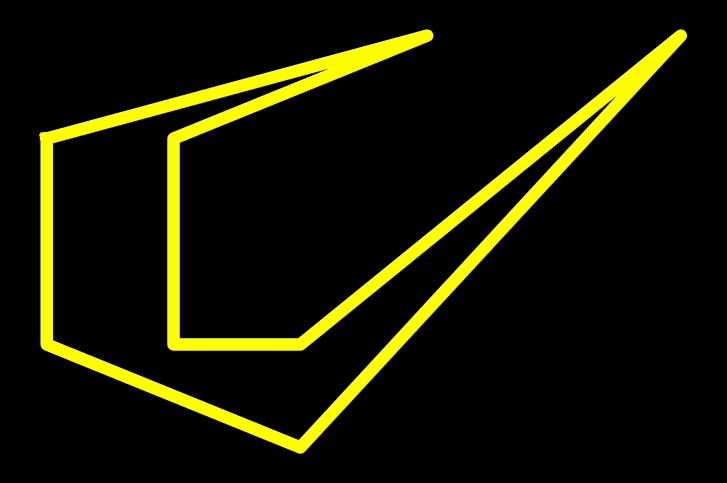
\includegraphics[width=2.5cm]{preface/vector_images/vec_image_curs1.png}
    
\includegraphics[width=2.5cm]{preface/vector_images/vec_image_curs2.png}
    
\includegraphics[width=2.5cm]{preface/vector_images/vec_image_curs3.png}
    
\includegraphics[width=2.5cm]{preface/vector_images/vec_image_curs4.png}
    
\includegraphics[width=2.5cm]{preface/vector_images/vec_image_curs5.png}
    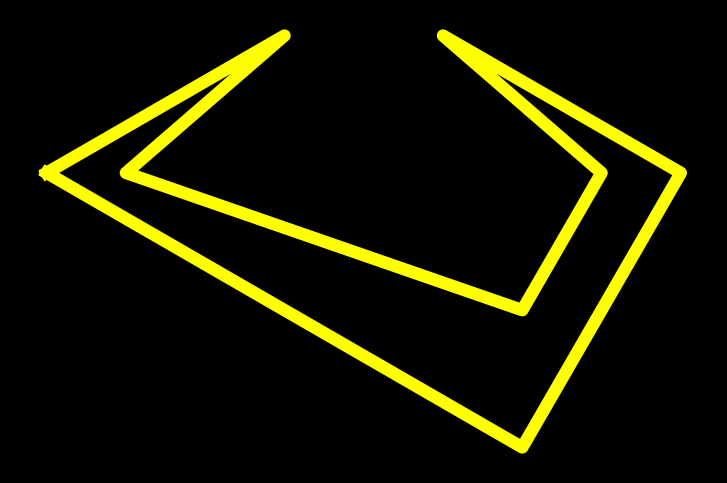
\includegraphics[width=2.5cm]{preface/vector_images/vec_image_curs6.png}
    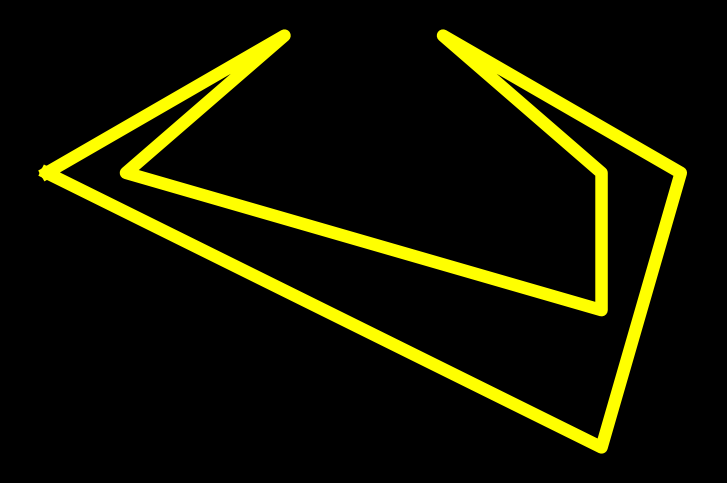
\includegraphics[width=2.5cm]{preface/vector_images/vec_image_curs7.png}
    
\includegraphics[width=2.5cm]{preface/vector_images/vec_image_curs8.png}
    
\includegraphics[width=2.5cm]{preface/vector_images/vec_image_ener11.png}
    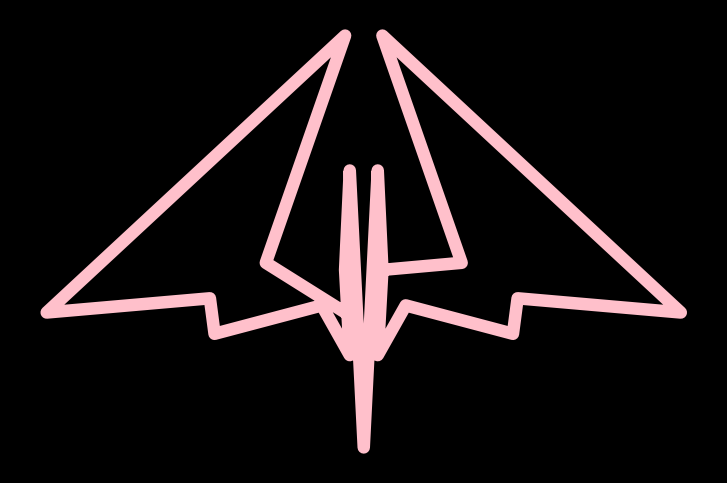
\includegraphics[width=2.5cm]{preface/vector_images/vec_image_ener12.png}
    
\includegraphics[width=2.5cm]{preface/vector_images/vec_image_ener13.png}
    
\includegraphics[width=2.5cm]{preface/vector_images/vec_image_ener14.png}
    
\includegraphics[width=2.5cm]{preface/vector_images/vec_image_ener21.png}
    
\includegraphics[width=2.5cm]{preface/vector_images/vec_image_ener22.png}
    
\includegraphics[width=2.5cm]{preface/vector_images/vec_image_ener23.png}
    
\includegraphics[width=2.5cm]{preface/vector_images/vec_image_ener24.png}
    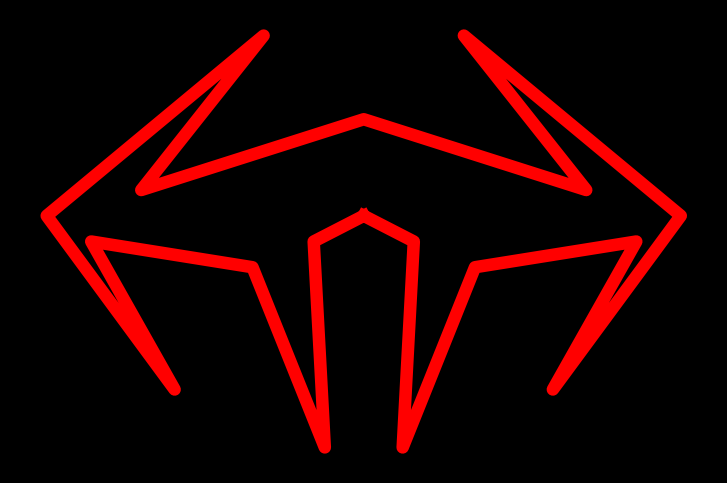
\includegraphics[width=2.5cm]{preface/vector_images/vec_image_ener41.png}
    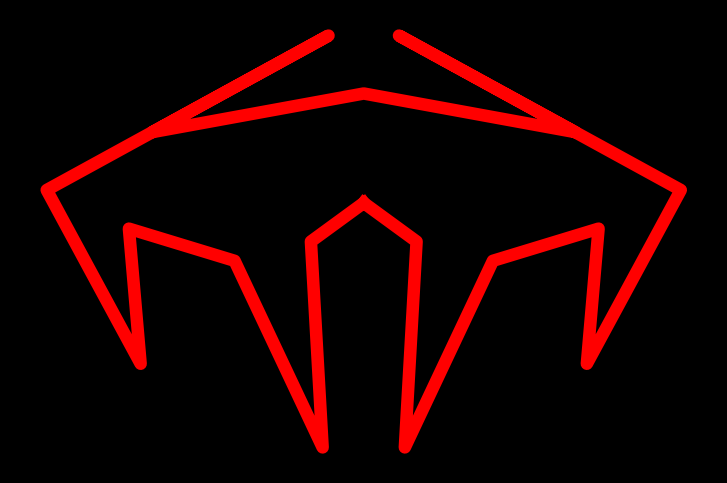
\includegraphics[width=2.5cm]{preface/vector_images/vec_image_ener42.png}
    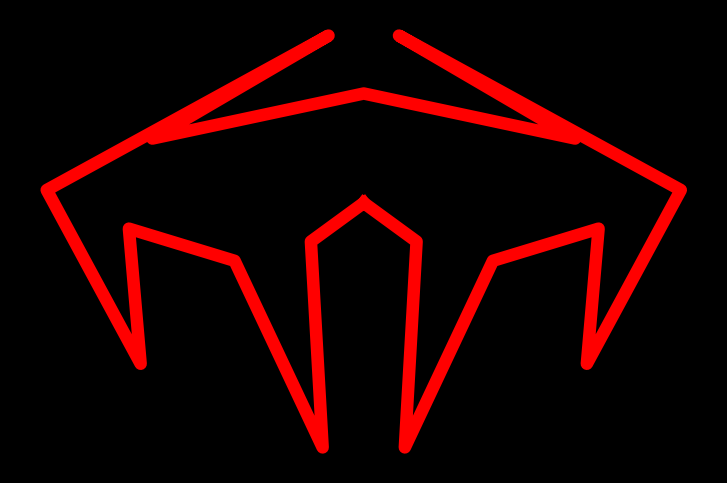
\includegraphics[width=2.5cm]{preface/vector_images/vec_image_ener43.png}
    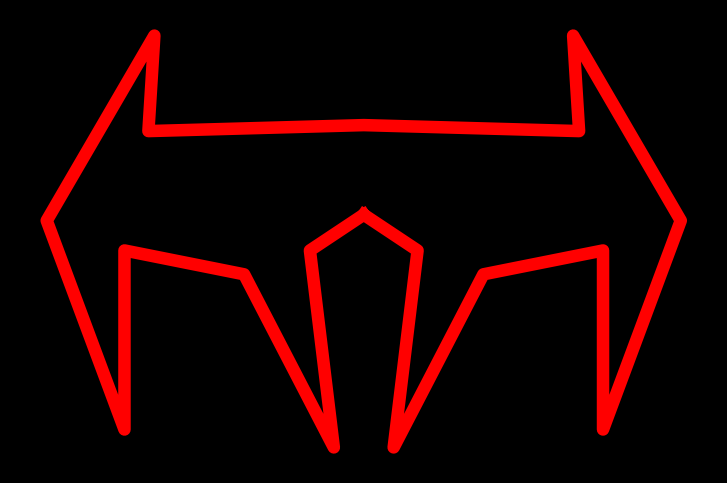
\includegraphics[width=2.5cm]{preface/vector_images/vec_image_ener44.png}
    
\includegraphics[width=2.5cm]{preface/vector_images/vec_image_expl1.png}
    
\includegraphics[width=2.5cm]{preface/vector_images/vec_image_explop.png}
    
\includegraphics[width=2.5cm]{preface/vector_images/vec_image_flipper.png}
    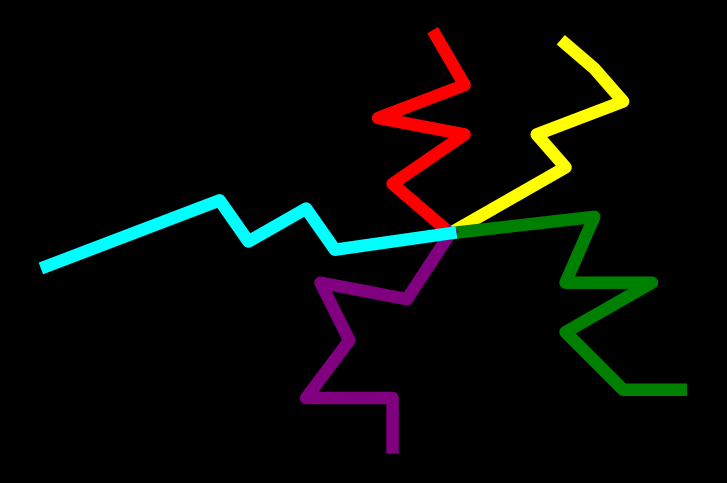
\includegraphics[width=2.5cm]{preface/vector_images/vec_image_fuse0.png}
    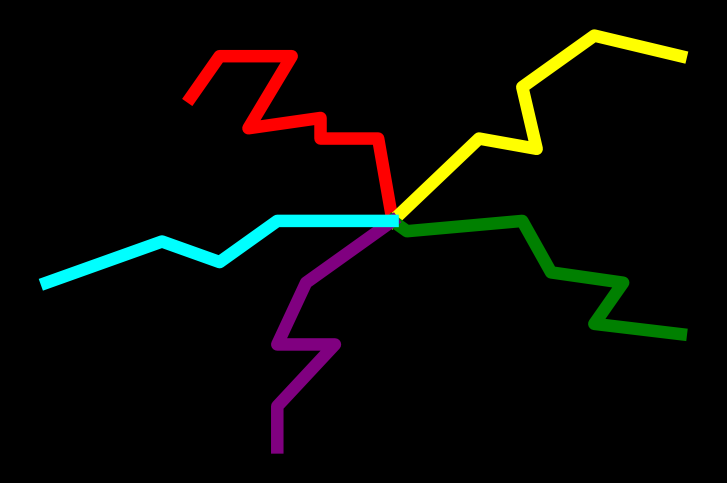
\includegraphics[width=2.5cm]{preface/vector_images/vec_image_fuse1.png}
    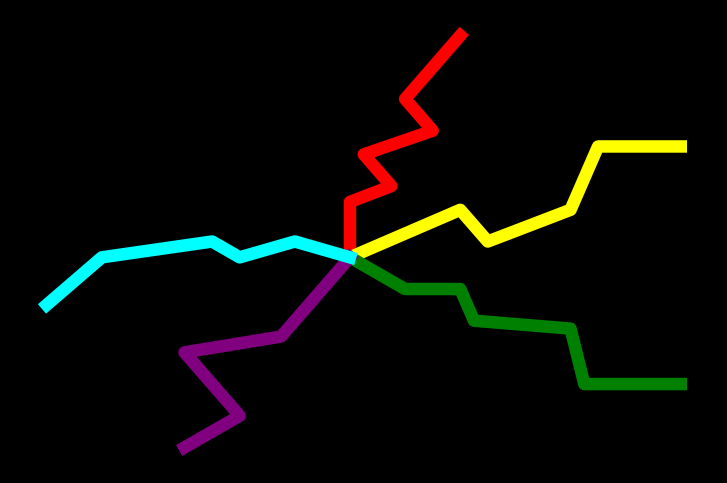
\includegraphics[width=2.5cm]{preface/vector_images/vec_image_fuse2.png}
    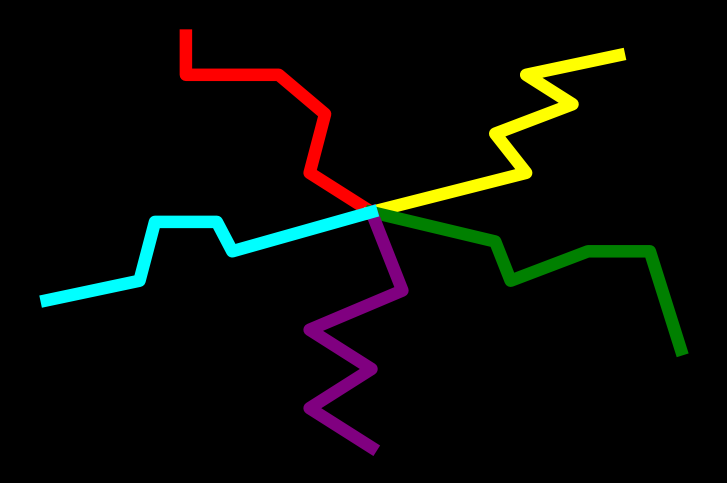
\includegraphics[width=2.5cm]{preface/vector_images/vec_image_fuse3.png}
    
\includegraphics[width=2.5cm]{preface/vector_images/vec_image_lifey.png}
    
\includegraphics[width=2.5cm]{preface/vector_images/vec_image_msauce.png}
    
\includegraphics[width=2.5cm]{preface/vector_images/vec_image_puls1.png}
    
\includegraphics[width=2.5cm]{preface/vector_images/vec_image_puls2.png}
    
\includegraphics[width=2.5cm]{preface/vector_images/vec_image_puls3.png}
    
\includegraphics[width=2.5cm]{preface/vector_images/vec_image_puls4.png}
    
\includegraphics[width=2.5cm]{preface/vector_images/vec_image_sa2pic.png}
    
\includegraphics[width=2.5cm]{preface/vector_images/vec_image_sa3pic.png}
    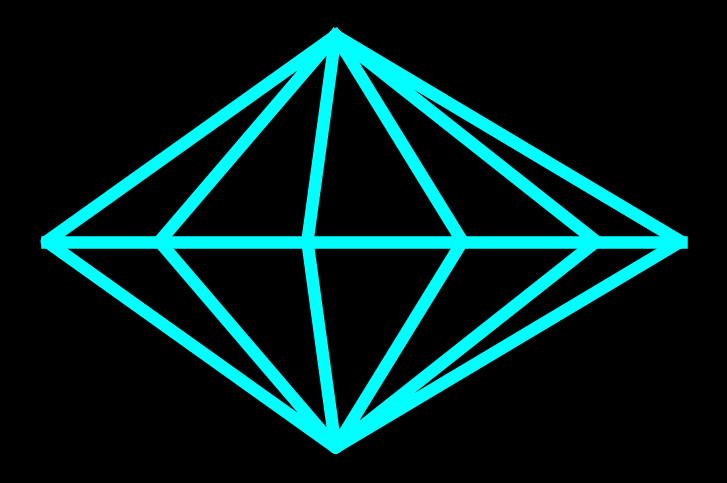
\includegraphics[width=2.5cm]{preface/vector_images/vec_image_sa4pic.png}
    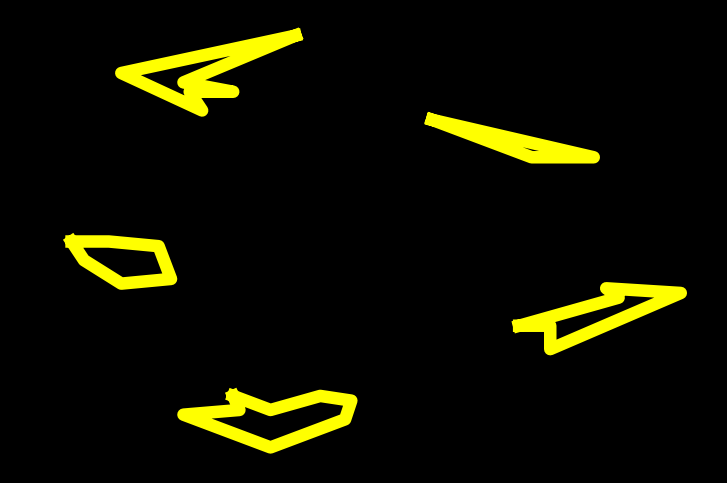
\includegraphics[width=2.5cm]{preface/vector_images/vec_image_shrap.png}
    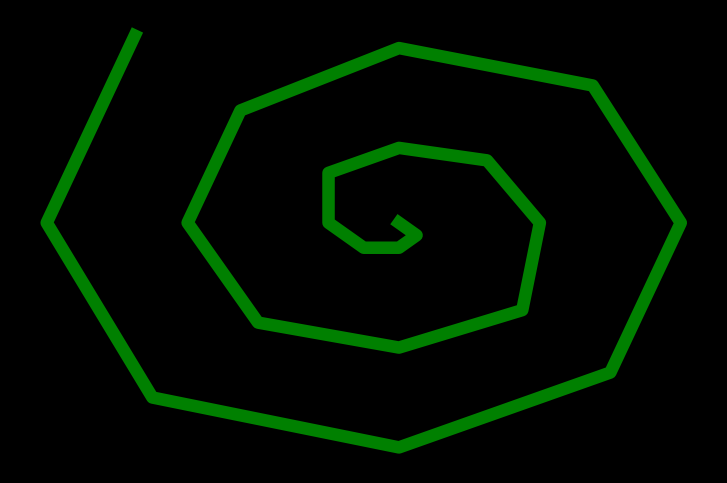
\includegraphics[width=2.5cm]{preface/vector_images/vec_image_spira1.png}
    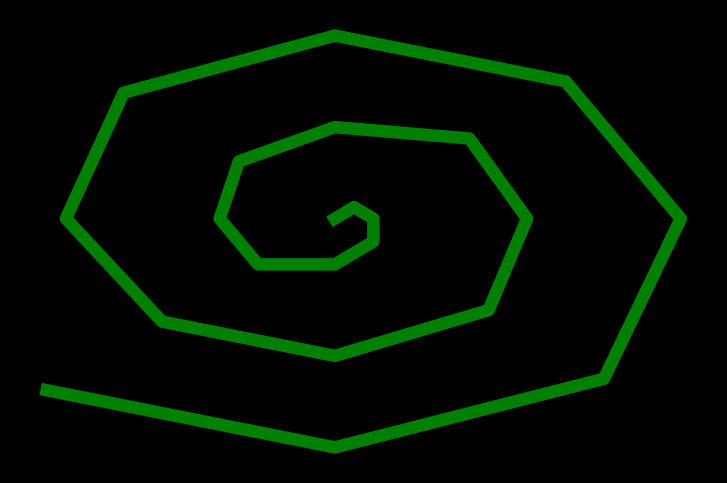
\includegraphics[width=2.5cm]{preface/vector_images/vec_image_spira2.png}
    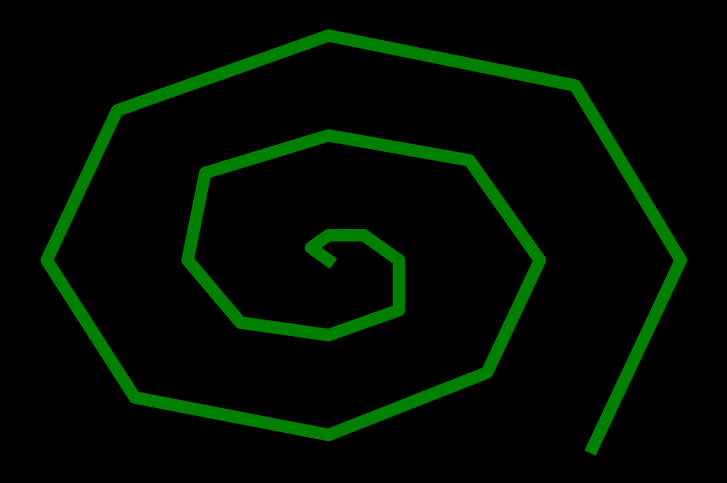
\includegraphics[width=2.5cm]{preface/vector_images/vec_image_spira3.png}
    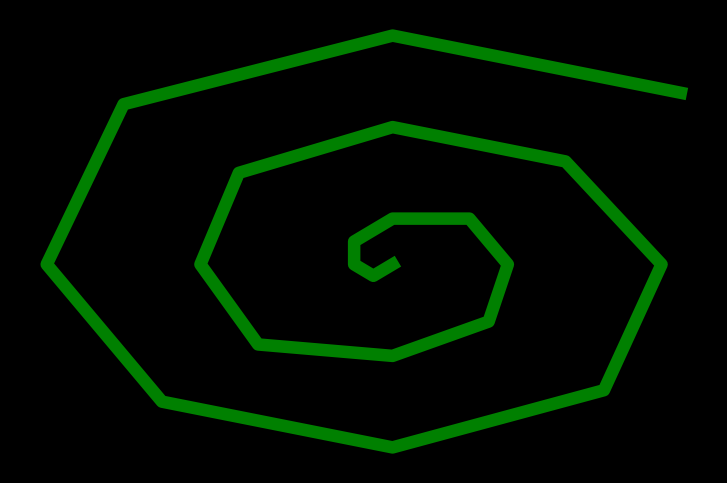
\includegraphics[width=2.5cm]{preface/vector_images/vec_image_spira4.png}
    
\includegraphics[width=2.5cm]{preface/vector_images/vec_image_splat.png}
    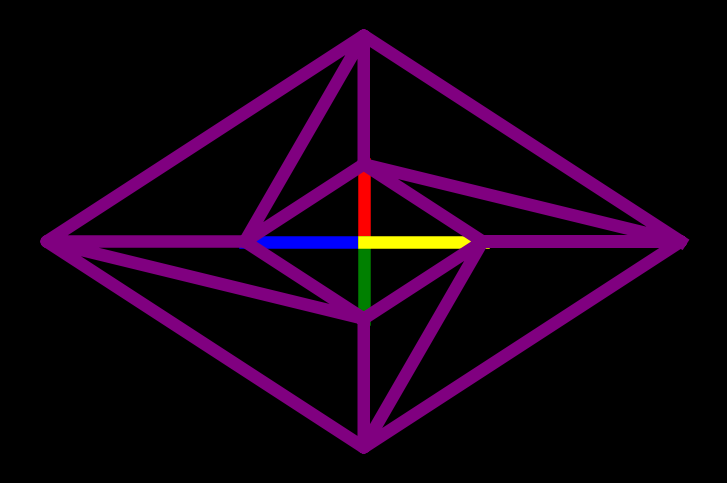
\includegraphics[width=2.5cm]{preface/vector_images/vec_image_tankf.png}
    
\includegraphics[width=2.5cm]{preface/vector_images/vec_image_tankp.png}
    
\includegraphics[width=2.5cm]{preface/vector_images/vec_image_tankr.png}
  \caption*{Artefacts from Tempest (1981).}
\end{figure}
\vspace*{\fill}
\thispagestyle{empty}% Turn off page number
\clearpage

\chapter*{about tempest and tempest 2000} 
\textit{Tempest} was a coin-operated arcade game released in 1981 by Atari
Corporation. At the time, its graphics and gameplay were at the very edge of
what was possible with contemporary hardware.  Its unique appearance was in
part attributable to its use of vector graphics, a technology that
drew lines of color, rather than pixels, on the screen and enabled the earliest
3D graphics in the arcade games of the time.

Some 15 years later, its successor \textit{Tempest 2000} was likewise a classic
game. To its misfortune it was made for a console that crashed and burned with
no survivors, and very few customers. The Jaguar was supposed to be Atari Corporation's first great
leap into the 64 bit era. Instead it promptly tripped over its shoelaces and
left a number of great games, Tempest 2000 among them, behind as orphans.

This book isn't about the history of \textit{Tempest} or its importance in the history
of computer games.  This is a book about computer code. Each chapter aims to be
an easily digested sketch of how a specific feature or effect was achieved. In
the case of \textit{Tempest} this means sifting through the 6502 assembly code
David Theurer wrote by hand(!) to create the game, and wrangling with the bits
and bytes of Atari's Quadrascan Vector Graphics. For \textit{Tempest 2000} it
means familiarizing ourselves with Motorola 68K assembly code and the Jaguar's
powerful hardware platform.

There are lots of fascinating bits and pieces to pore over. And it is
interesting to see how the years that separate the two games leave some things
unchanged and many other things changed utterly. I've put together this book of
squibs in the hope they will allow you, the reader, to digest small bite-sized
insights into each game. And I hope, by interleaving elements from \textit{Tempest} and
\textit{Tempest 2000}, to enable you to compare the parallel lives in the design
and execution of separate incarnations of the same classic video game.

Rob Hogan (\href{https://mastodon.social/@mwenge}{\textcolor{blue}{@mwenge}})\\
\the\year{} \\

\thispagestyle{empty}% Turn off page number
\clearpage
\vspace*{\fill}
\begin{figure}[H]
  \centering

\includegraphics[width=2.5cm]{preface/obj2d/obj_0.png}
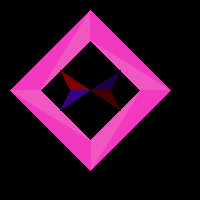
\includegraphics[width=2.5cm]{preface/obj2d/obj_1.png}
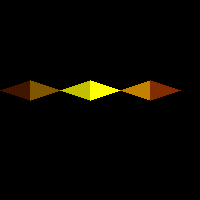
\includegraphics[width=2.5cm]{preface/obj2d/obj_10.png}

\includegraphics[width=2.5cm]{preface/obj2d/obj_13.png}

\includegraphics[width=2.5cm]{preface/obj2d/obj_14.png}
\includegraphics[width=2.5cm]{preface/obj2d/obj_15.png}
\includegraphics[width=2.5cm]{preface/obj2d/obj_16.png}
\includegraphics[width=2.5cm]{preface/obj2d/obj_17.png}
\includegraphics[width=2.5cm]{preface/obj2d/obj_18.png}
\includegraphics[width=2.5cm]{preface/obj2d/obj_19.png}
\includegraphics[width=2.5cm]{preface/obj2d/obj_2.png}
\includegraphics[width=2.5cm]{preface/obj2d/obj_20.png}
\includegraphics[width=2.5cm]{preface/obj2d/obj_21.png}
\includegraphics[width=2.5cm]{preface/obj2d/obj_22.png}
\includegraphics[width=2.5cm]{preface/obj2d/obj_23.png}
\includegraphics[width=2.5cm]{preface/obj2d/obj_24.png}
\includegraphics[width=2.5cm]{preface/obj2d/obj_25.png}
\includegraphics[width=2.5cm]{preface/obj2d/obj_26.png}
\includegraphics[width=2.5cm]{preface/obj2d/obj_27.png}
\includegraphics[width=2.5cm]{preface/obj2d/obj_28.png}
\includegraphics[width=2.5cm]{preface/obj2d/obj_29.png}
\includegraphics[width=2.5cm]{preface/obj2d/obj_3.png}
\includegraphics[width=2.5cm]{preface/obj2d/obj_30.png}
\includegraphics[width=2.5cm]{preface/obj2d/obj_31.png}
\includegraphics[width=2.5cm]{preface/obj2d/obj_4.png}
\includegraphics[width=2.5cm]{preface/obj2d/obj_5.png}
\includegraphics[width=2.5cm]{preface/obj2d/obj_6.png}
\includegraphics[width=2.5cm]{preface/obj2d/obj_7.png}
\includegraphics[width=2.5cm]{preface/obj2d/obj_8.png}
\includegraphics[width=2.5cm]{preface/obj2d/obj_9.png}
  \caption*{Artefacts from Tempest 2000 (1994).}
\end{figure}
\vspace*{\fill}
\thispagestyle{empty}% Turn off page number
\clearpage
\vspace*{\fill}
\begin{figure}[H]
    \centering
      \includegraphics[width=9cm]{src/cover/title_page.png}%
\end{figure}
\vspace*{\fill}
\thispagestyle{empty}% Turn off page number
\clearpage % Makes sure no header rule on last page

